\begin{adjustwidth*}{}{-2.25in}
\textbf{{\large Exercises}}
\setlength{\columnsep}{25pt}
\begin{multicols*}{2}
\noindent Terms and Concepts \small

\begin{enumerate}[1)]
\item {T/F: If $\ds \lim_{x\to 5} f(x) = \infty$, then we are implicitly stating that the limit exists.}
\item {T/F: If $\ds \lim_{x\to \infty} f(x) = 5$, then we are implicitly stating that the limit exists.}
\item {T/F: If $\ds \lim_{x\to 1^-} f(x) = -\infty$, then $\ds \lim_{x\to 1^+} f(x) = \infty$}
\item {T/F: If $\ds \lim_{x\to 5} f(x) = \infty$, then $f$ has a vertical asymptote at $x=5$.}
\item {T/F: $\infty/0$ is not an indeterminate form.}
\item {Construct a function with a vertical asymptote at $x=5$ and a horizontal asymptote at $y=5$.}
%\item {Let $\ds \lim_{x\to 7} f(x) = \infty$. Explain how we know that $f$ is/is not continuous at $x=7$.}
\end{enumerate} 

\noindent {\normalsize Problems\\} \small

\noindent In exercises 7--12, evaluate each limit using the given graph of $f(x)$.

\begin{enumerate}[1),resume]
\item 
{$\ds f(x) = \frac{1}{(x+1)^2}$
\begin{enumerate}
\item		$\ds \lim_{x\to -1^-} f(x)$
\item		$\ds \lim_{x\to -1^+} f(x)$
\end{enumerate}

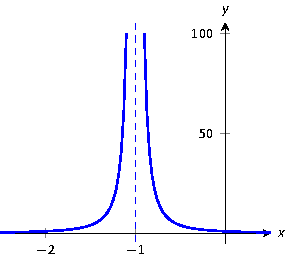
\includegraphics[scale=.8]{figures/fig01_06_ex_09}
}

\item
{$\ds f(x) = \frac{1}{(x-3)(x-5)^2}$.

\begin{minipage}[t]{.5\linewidth}
\begin{enumerate}
\item		$\ds \lim_{x\to 3^-} f(x)$
\item		$\ds \lim_{x\to 3^+} f(x)$
\item		$\ds \lim_{x\to 3} f(x)$
\end{enumerate}
\end{minipage}
\begin{minipage}[t]{.5\linewidth}
\begin{enumerate}\addtocounter{enumii}{3}
\item		$\ds \lim_{x\to 5^-} f(x)$
\item		$\ds \lim_{x\to 5^+} f(x)$
\item		$\ds \lim_{x\to 5} f(x)$
\end{enumerate}
\end{minipage}

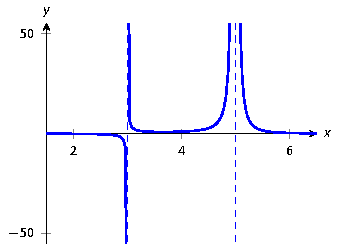
\includegraphics[scale=.8]{figures/fig01_06_ex_10}
}

\item
{$\ds f(x) = \frac{1}{e^x+1}$

\begin{minipage}[t]{.5\linewidth}
\begin{enumerate}
\item		$\ds \lim_{x\to -\infty} f(x)$
\item		$\ds \lim_{x\to \infty} f(x)$
\end{enumerate}
\end{minipage}
\begin{minipage}[t]{.5\linewidth}
\begin{enumerate}\addtocounter{enumii}{2}
\item		$\ds \lim_{x\to 0^-} f(x)$
\item		$\ds \lim_{x\to 0^+} f(x)$
\end{enumerate}
\end{minipage}

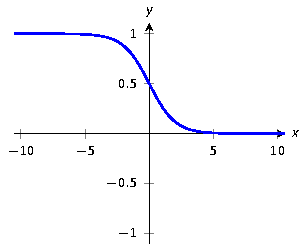
\includegraphics[scale=.8]{figures/fig01_06_ex_11}
}

\item
{$\ds f(x) = x^2\sin (\pi x)$

\begin{enumerate}
\item		$\ds \lim_{x\to -\infty} f(x)$
\item		$\ds \lim_{x\to \infty} f(x)$
\end{enumerate}

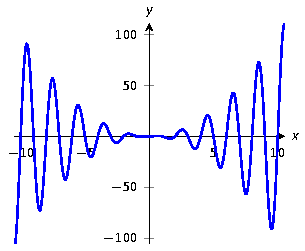
\includegraphics[scale=.8]{figures/fig01_06_ex_12}
}

\item
{$\ds f(x) = \cos (x)$

\begin{enumerate}
\item		$\ds \lim_{x\to -\infty} f(x)$
\item		$\ds \lim_{x\to \infty} f(x)$
\end{enumerate}

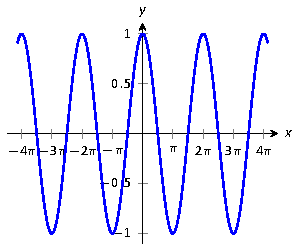
\includegraphics[scale=.8]{figures/fig01_06_ex_13}
}

\item
{$\ds f(x) = 2^x+10$
\begin{enumerate}
\item		$\ds \lim_{x\to -\infty} f(x)$
\item		$\ds \lim_{x\to \infty} f(x)$
\end{enumerate}

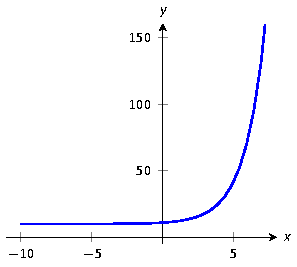
\includegraphics[scale=.8]{figures/fig01_06_ex_40}
}

\end{enumerate}

\vspace{.5cm}

%------------------------------------------
% END OF EXERCISES ON FIRST PAGE
%------------------------------------------
\end{multicols*}
\end{adjustwidth*}

\clearpage

\begin{adjustwidth*}{}{-2.25in}
\setlength{\columnsep}{25pt}
\begin{multicols*}{2}\small

In exercises 13--23, evaluate the limit.

\begin{multicols}{2}
\begin{enumerate}[1),start=13]
\item {$\ds \lim_{x \to -3^+} \frac{x-2}{x+3}$}
\item {$\ds \lim_{x \to 5^-} \frac{4}{x-5}$}
\item {$\ds \lim_{x \to 1} \frac{3-x}{(x-1)^2}$}
\item {$\ds \lim_{x \to \pi^-} \cot(x)$}
\item {$\ds \lim_{x\to\infty} \frac{x^3+2x^2+1}{5-x}$}
\item {$\ds \lim_{x\to-\infty} \frac{x^3+2x^2+1}{x^2-5}$}
\item {$\ds \lim_{x\to-\infty} \frac{x^3+2x^2+1}{5-x^2}$}
\item {$\ds \lim_{x \to \infty} \left( x - \sqrt{x} \right)$}
\item $\ds \lim_{x \to \infty} \frac{x+2}{\sqrt{9x^2 + 8}}$
\item $\ds \lim_{x \to -\infty} \frac{\sin^2(x)}{x^2}$
\item $\ds \lim_{x \to -\infty} \left( x^4 + x^5 \right)$
\end{enumerate}
\end{multicols}

\vspace{.5cm}

%---------------------------------------------
% END OF EXERCISES ON SECOND PAGE
%---------------------------------------------
\end{multicols*}
\end{adjustwidth*}
\afterexercises